\documentclass[a4paper,twocolumn,11pt,nopdfoutputerror]{quantumarticle}
\ifdefined\pdfoutput\pdfoutput=1\fi
\usepackage[T1]{fontenc}
\usepackage[utf8]{inputenc}
\usepackage{amsmath,amssymb,amsthm,bm,booktabs,graphicx,listings,tabularx}
\usepackage{microtype}
\newcommand{\R}{\mathbb{R}}
\newcommand{\I}{\mathbb{I}}
\newcommand{\tr}{\operatorname{tr}}
\newcommand{\diag}{\operatorname{diag}}
\newcommand{\CZ}{\operatorname{CZ}}
\newcommand{\Var}{\operatorname{Var}}
\newcommand{\Cov}{\operatorname{Cov}}
\newtheorem{proposition}{Proposition}
\lstset{basicstyle=\ttfamily\scriptsize,breaklines=true,columns=fullflexible,frame=single}
\title{PhotoGraphiQ}
\author{PhotoGraphiQ contributors}
\affiliation{Software manuscript draft; individual authors and affiliations to be confirmed.}
\date{10 September 2026}

\begin{document}
\maketitle

\begin{abstract}
PhotoGraphiQ is an open-source Python framework for continuous-variable photonic
measurement-based quantum computing. It separates weighted graph resources,
measurement patterns, real-valued classical dependencies, Gaussian compilation,
and physical simulation. Piquasso supplies photonic gate execution; an independent
phase-space backend and an affine channel analyzer provide complementary numerical
checks. The framework supports finite squeezing, adaptive quadrature measurements,
general Gaussian measurements, displacement feed-forward, causal validation,
numerical CV-flow certificates for specified measurement orders, serialization,
and visualization. A Gaussian compiler constructs teleportation patterns for
single-mode symplectic gates and two-mode interactions, while an experimental
Fock adapter supports explicitly truncated non-Gaussian resources and conditional
photon counting. We derive the conventions, measurement updates, teleportation
noise, compiler factorization, and displacement-frame rules used by the software.
Validation distinguishes analytical physics, raw Piquasso comparisons, and
structural comparisons with the qubit MBQC framework GraphiX. Reproducible
finite-squeezing data illustrate the difference between conditional trajectories
and unconditional channels. The release targets transparent, testable Gaussian
MBQC and resource experiments; it does not claim universal non-Gaussian
compilation, automatic differentiation, or fault-tolerant photonic computation.
\end{abstract}

\section{Introduction}

Measurement-based quantum computing (MBQC) encodes a computation in an entangled
resource and a sequence of measurements and classical corrections. In the
continuous-variable (CV) setting, bosonic modes replace qubits, quadrature
measurements produce real-valued outcomes, and physical graph resources have
finite squeezing. These differences affect both the mathematics of computation
and the structure of a useful software interface. CV cluster computation and its
Gaussian and non-Gaussian resources have well-established theoretical
foundations~\cite{menicucci2006,gu2009}. A software implementation must make its
finite-resource and convention choices explicit rather than inherit binary
measurement rules from a qubit implementation.

Piquasso provides photonic circuit simulation in Gaussian and Fock
representations~\cite{piquasso2025}. GraphiX provides an architectural reference for
qubit measurement patterns, command manipulation and simulation~\cite{graphix2022}.
PhotoGraphiQ occupies the layer between these capabilities: its primary objects
are graph resources and adaptive measurement computations, and its backend
translates their physical operations into photonic simulation. The intended
extension path is Piquasso $\rightarrow$ PhotoGraphiQ $\rightarrow$ a future
PhotoGraphiQML package. No machine-learning dependencies are introduced in the
present runtime.

\subsection{Contributions and assumptions}

This article describes the implemented version 0.1.0 repository. Its contributions
are a backend-independent command representation with causal classical signals;
finite-squeezing Gaussian graph preparation and exact destructive measurement
conditioning; a teleportation-based Gaussian compiler; independent unconditional
channel analysis; specified-order CV-flow certification; a conservative
displacement frame and rewrite system; and a validation suite with reproducible
examples and data. We additionally expose a bounded experimental Fock backend.

The assumptions are explicit. Gaussian trajectories use dense first and second
moments with $\hbar=2$. Gaussian compilation implements noisy finite-resource
channels whose ideal symplectic targets are checked separately. The Fock adapter
uses a global total-photon cutoff and does not support adaptive homodyne
conditioning. CV-flow is checked for a supplied total order; the software does
not search for maximally parallel flow. A dependency DAG by itself is not a
determinism certificate. GraphiX validates corresponding structures, not equality
between CV and qubit states.

The work is a software implementation and validation report. It does not claim a
new teleportation identity, new Gaussian compilation theorem, experimental
photonic data, or a performance advantage over existing simulation libraries.
The manuscript is a draft for author review, not a statement of publication or
acceptance by \emph{Quantum}.

\section{Architecture and computational objects}
\label{sec:architecture}

The package uses a \texttt{src/photographiq} layout. Graph topology, commands,
expressions and measurement descriptions do not contain Piquasso instructions.
The execution engine resolves classical values and calls an abstract backend.
Backend state is kept separate from the pattern, so the same computation can be
executed repeatedly with different inputs, parameters or random seeds.

\begin{table*}[t]
\centering\small
\begin{tabularx}{\textwidth}{p{.18\textwidth}p{.29\textwidth}X}
\toprule
Layer & Principal modules & Responsibility \\
\midrule
Resource & \texttt{graph}, \texttt{states} & Weighted topology, node roles, Gaussian/Fock inputs \\
Intermediate representation & \texttt{commands}, \texttt{pattern} & Ordered physical and classical instructions \\
Measurement calculus & \texttt{measurements}, \texttt{expressions} & POVM descriptions, parameter and outcome dependencies \\
Causality and flow & \texttt{flow}, \texttt{cvflow} & Command scheduling and distinct real-linear flow certificates \\
Compilation & \texttt{compiler}, \texttt{protocols} & Teleportation gadgets and Gaussian circuit translation \\
Execution & \texttt{simulator}, \texttt{backends} & Conditional trajectories, frames and native gates \\
Analysis & \texttt{gaussian}, \texttt{analysis} & Symplectic identities and unconditional Gaussian channels \\
Interchange & \texttt{serialization}, \texttt{visualization} & Allowlisted JSON and resource/dependency figures \\
Research artifacts & \texttt{tests}, \texttt{examples}, \texttt{experiments}, \texttt{docs}, \texttt{paper} & Validation, tutorials, data and manuscript \\
\bottomrule
\end{tabularx}
\caption{Repository organization. The Gaussian measurement adapter is shared by
the two Gaussian execution backends; the independent channel analyzer and
analytical tests supply additional validation.}
\label{tab:modules}
\end{table*}

\subsection{Graphs and node roles}

\texttt{CVGraph} wraps an undirected simple weighted graph. Vertices have stable
labels and resource squeezing, while edges have real coupling weights. Input and
output tuples preserve user ordering. Ancillas are non-input nodes; measured
nodes are identified by a pattern's measurement commands. Directed resources,
multiedges, self-loops and nonfinite numerical weights are rejected. A diagonal
quadratic phase is a local operation rather than a self-edge in this resource
model.

Constructors cover lines, rings, stars, trees, rectangular and square lattices,
adjacency matrices and arbitrary NetworkX graphs. Temporal resources currently
mean time-labelled line topology, and the dual-rail constructor means a ladder
graph. These names do not assert that an experimental time-multiplexed
interferometer has been synthesized. Figure~\ref{fig:resource} illustrates the
labelled-resource view.

\begin{figure}[t]
\centering
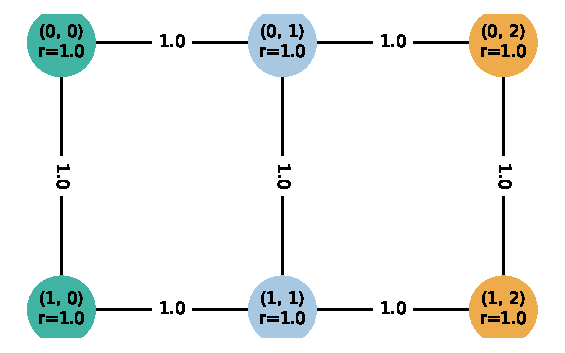
\includegraphics[width=\columnwidth]{results/resource.pdf}
\caption{An exported two-row resource. Labels, squeezing and weights belong to
the resource description. Green and amber nodes denote inputs and outputs;
measurements and dependencies are added at the pattern layer.}
\label{fig:resource}
\end{figure}

\subsection{Patterns, commands and execution}

The command vocabulary consists of preparation, entanglement, measurement,
displacement, rotation, squeezing, beam splitter, loss, cubic phase, classical
signal and output declaration. A pattern can be constructed from a graph or by
appending commands. Input modes are supplied separately and cannot be prepared
again. A measurement removes its mode and writes a result under a unique key;
the default key is the node label. An optional final output declaration can
select or reorder survivors, tracing out other modes.

The execution sequence is
\begin{equation}
 \begin{aligned}
 &\text{command}\to\text{resolve values}\to\text{backend}\\
 &\hspace{2em}\to\text{record outcome}\to\text{next command}.
 \end{aligned}
\end{equation}
This is a genuinely adaptive sequence: later measurements may depend on earlier
real outcomes. \texttt{Result} stores measurement outcomes, all classical records,
an independent output-state snapshot, backend identity and seed information.
The pattern itself is not mutated by simulation.

\subsection{Expression safety and causality}

An external \texttt{Parameter} and a previous \texttt{Outcome} are distinct
expression leaves. Arithmetic and a small set of elementary functions construct
an expression tree. Runtime resolution requires finite real scalar values.
Vector-valued general-dyne outcomes are accessed by an explicit component.
\texttt{Signal} commands create named intermediate classical registers.

Callables are permitted through a wrapper with declared dependencies. The
function receives only those records, so undeclared access fails even if the
record happens to exist. Callables cannot be serialized. The portable expression
language uses neither Python string evaluation nor arbitrary code deserialization.

Causal validation creates one graph vertex per command, inserts producer-to-user
edges for classical records, and preserves consecutive touches of each quantum
mode. It rejects missing producers, duplicate keys, cycles, future dependencies,
double preparation, and operations on measured modes. Topological scheduling
then provides a legal command order under these constraints. It is not a search
for a different measurement calculus or a proof of ideal-limit convergence.

\section{Phase-space conventions}
\label{sec:conventions}

The internal quadrature vector and commutators are
\begin{equation}
 \bm R=(q_0,p_0,q_1,p_1,\ldots)^T,\qquad
 [R_j,R_k]=2i\Omega_{jk},
\end{equation}
where $\Omega=\bigoplus_j\left(\begin{smallmatrix}0&1\\-1&0\end{smallmatrix}\right)$.
Means and statistical covariance are
\begin{equation}
 \bm\mu=\langle\bm R\rangle,\qquad
 V_{jk}=\tfrac12\langle\{\Delta R_j,\Delta R_k\}\rangle.
\end{equation}
Vacuum has $V=\I$ and Gaussian physicality requires $V+i\Omega\succeq0$.
The state validator checks dimensions, labels, finiteness, symmetry and this
uncertainty condition with a documented numerical tolerance.

Piquasso's covariance convention is the unhalved anticommutator matrix
$\sigma=2V$. Thus native covariance and displacement units are converted at the
backend boundary. The real symplectic matrices for rotation and squeezing are
\begin{align}
 R(\phi)&=\begin{pmatrix}\cos\phi&-\sin\phi\\\sin\phi&\cos\phi\end{pmatrix},\\
 S(r)&=\diag(e^{-r},e^r).
\end{align}
Positive gate squeezing reduces $q$ variance. Positive \emph{resource} squeezing
$r$ instead means preparation with $S(-r)$, reducing $p$ variance.

The controlled-phase and translation conventions are
\begin{align}
 \CZ_{ij}(g)&=e^{igq_iq_j/2},\label{eq:cz}\\
 X(s)&=e^{-isp/2},\qquad Z(t)=e^{itq/2}.
\end{align}
Equation~\eqref{eq:cz} sends $p_i\mapsto p_i+gq_j$ and
$p_j\mapsto p_j+gq_i$. The translations shift $q$ and $p$ by $s$ and $t$;
Piquasso's complex displacement is therefore $\alpha=(s+it)/2$.
No angle in the public interface is implicitly measured in units of $\pi$.

\section{Finite-squeezing graph resources}

For a symmetric zero-diagonal adjacency matrix $A$, prepare independent
momentum-squeezed modes and apply the product of weighted CZ gates. In grouped
coordinate order $(\bm q,\bm p)$, let
\begin{equation}
 D_q=\diag(e^{2r_j}),\qquad D_p=\diag(e^{-2r_j}).
\end{equation}
The graph symplectic map and covariance are
\begin{align}
 S_A&=\begin{pmatrix}\I&0\\A&\I\end{pmatrix},\\
 V_A&=\begin{pmatrix}D_q&D_qA\\AD_q&D_p+AD_qA\end{pmatrix}.
 \label{eq:graphcov}
\end{align}
The implementation stores these matrices in interleaved order.

\begin{proposition}
The nullifiers $\bm\delta=\bm p-A\bm q$ of the resource in
Eq.~\eqref{eq:graphcov} commute and have covariance $D_p$.
\end{proposition}
\begin{proof}
Symmetry of $A$ cancels the commutators between the two linear terms. Under
$S_A$, $\bm p-A\bm q$ is the original independent squeezed momentum vector.
Its covariance is consequently $D_p$.
\end{proof}

The nullifier identity provides a sensitive test of edge signs, squeezing axes,
coordinate order and covariance factors. Arbitrary input states can replace the
designated input preparations, including correlated Gaussian inputs. The simple
resource-only nullifier covariance must then be interpreted with the actual
input state rather than reused without qualification.

An ideal symbolic graph retains topology and nullifier coefficients but cannot
be executed as a finite covariance state. Infinite squeezing is not encoded by
overflowing floating-point values. Piquasso's native \texttt{Graph} preparation
is not used as a substitute for the canonical resource in Eq.~\eqref{eq:graphcov}.

\section{Measurements and classical adaptation}

\subsection{Exact homodyne conditioning}

Partition the measured mode and the survivors as
\begin{equation}
 \bm\mu=\begin{pmatrix}\bm b\\\bm a\end{pmatrix},\qquad
 V=\begin{pmatrix}B&C^T\\C&A\end{pmatrix}.
\end{equation}
For $h=(\cos\theta,\sin\theta)$, homodyne measures $y=h\bm R_m$.
With nonnegative calibrated detector noise $\nu$, define
\begin{equation}
 v=hBh^T+\nu,\qquad y\sim\mathcal N(h\bm b,v).
\end{equation}
The conditional survivor state is
\begin{align}
 \bm\mu'&=\bm a+Ch^T\frac{y-h\bm b}{v},\label{eq:hommean}\\
 V'&=A-\frac{Ch^ThC^T}{v}.\label{eq:homcov}
\end{align}
An ideal detector uses $\nu=0$. Efficiency $0<\eta\leq1$ is modeled by vacuum
mixing followed by calibration to the incoming quadrature, yielding
$\nu=(1-\eta)/\eta+\nu_{\mathrm{readout}}$. The measured mode is removed.
Linear solves are used for matrix-valued conditioning; singular or invalid
requests raise errors.

\subsection{Heterodyne and general Gaussian measurements}

A general-dyne detector is represented by a physical statistical covariance
$M$, with $M+i\Omega_1\succeq0$. The outcome and update are
\begin{align}
 \bm y&\sim\mathcal N(\bm b,B+M),\\
 \bm\mu'&=\bm a+C(B+M)^{-1}(\bm y-\bm b),\\
 V'&=A-C(B+M)^{-1}C^T.
\end{align}
Heterodyne uses $M=\I$. It returns two phase-space coordinates, so its vacuum
outcome covariance is $2\I$ in the chosen units. These values should not be
confused with the real and imaginary parts of $\alpha=(q+ip)/2$.

\subsection{Native-backend convention audit}

Source inspection and tests exposed differences that are recorded in
\texttt{docs/design.md}. The inspected Piquasso ControlledZ Bogoliubov blocks
produce the positive momentum update used here, despite an opposite sign in
its displayed unitary docstring. Its Gaussian homodyne routine uses a
finite detector covariance $\diag(z^2,z^{-2})$, with $q$ homodyne approached
as $z\to0$.

More significantly, the pinned version 8.0.1 passes an anticommutator covariance
to its Gaussian random sampler without the statistical factor $1/2$. A separate
raw characterization test consequently observes vacuum heterodyne variance near
$4$ rather than $2$. PhotoGraphiQ does not silently inherit that sampling
convention. Piquasso performs native gates; PhotoGraphiQ performs the exact
Gaussian measurement adapter in Eqs.~\eqref{eq:hommean}--\eqref{eq:homcov} and
their general-dyne counterparts. Native conditional moments can still be checked
at native sample values; this tests the state update, not the physical sampling
distribution. Dependency versions are pinned so such behavior remains reviewable.

\section{Teleportation protocols and Gaussian compilation}

\subsection{Elementary cluster step}

Take an input mode and an independent momentum-squeezed ancilla. Apply unit CZ,
measure $m=p_0+kq_0$ on the input, and correct the ancilla by $X(-m)$. In terms
of the pre-entanglement variables, the resulting output relations are
\begin{equation}
 \begin{aligned}
 \bm R_{\mathrm{out}}&=T(k)\bm R_{\mathrm{in}}+(0,p_{\mathrm{anc}})^T,\\
 T(k)&=\begin{pmatrix}-k&-1\\1&0\end{pmatrix}.
 \end{aligned}
 \label{eq:step}
\end{equation}
Indeed, before the measurement the measured momentum is $p_0+q_1$, while
the surviving momentum is $p_1+q_0$. Subtracting the measured value from the
surviving position cancels $q_1$.

The physical measurement description is normalized: the software sets
$\theta=\operatorname{atan2}(1,k)$ and records
$y=q\cos\theta+p\sin\theta$. The feed-forward value is
$m=y/\sin\theta$, not $y$. This normalization is necessary for nonzero $k$.

\begin{proposition}
For Gaussian inputs, the outcome-averaged corrected channel of a cluster step is
\begin{equation}
 \begin{aligned}
 \bm\mu&\mapsto T(k)\bm\mu,\\
 V&\mapsto T(k)VT(k)^T+N_r,\\
 N_r&=\diag(0,e^{-2r}).
 \end{aligned}
 \label{eq:stepchannel}
\end{equation}
\end{proposition}
\begin{proof}
The input and ancilla variables in Eq.~\eqref{eq:step} are initially independent.
The ancilla momentum has zero mean and variance $e^{-2r}$. Taking unconditional
first and second moments gives Eq.~\eqref{eq:stepchannel}. Equivalently, Gaussian
Wigner-variable propagation integrates the homodyne-conditioned branches.
\end{proof}

This proposition is deliberately an unconditional statement. Finite-resource
conditional means and covariances depend on the observed branch. Averaging only
conditional covariance omits the covariance of the conditional means.

\subsection{Wires, identity and optical teleportation}

A single $k=0$ step is a Fourier transformation, $T(0)=R(\pi/2)$.
Four such steps implement identity with added covariance $2e^{-2r}\I$ for
uniform resources. For a general wire, the exact recursion is
\begin{align}
 S_j&=T(k_j)S_{j-1},\\
 N_j&=T(k_j)N_{j-1}T(k_j)^T+N_{r_j},\\
 S_0&=\I,\qquad N_0=0.
 \label{eq:noise}
\end{align}
The repository separately implements Braunstein--Kimble optical
teleportation~\cite{bk1998}. Oppositely squeezed resources, a balanced beam
splitter, complementary Bell homodynes and gain-$\sqrt2$ corrections produce
$V_{\mathrm{out}}=V_{\mathrm{in}}+2e^{-2r}\I$ in the ensemble. This optical
protocol is named separately from canonical CZ cluster propagation.

\subsection{Single-mode symplectic decomposition}

Let $S=\left(\begin{smallmatrix}A&B\\C&D\end{smallmatrix}\right)$ with
$AD-BC=1$. If $C\ne0$, the chronological list
\begin{equation}
 (k_1,k_2,k_3,k_4)=\left(0,\frac{1-D}{C},C,\frac{1-A}{C}\right)
 \label{eq:decomp}
\end{equation}
satisfies $S=T(k_4)T(k_3)T(k_2)T(k_1)$.
Multiplication gives the desired $A,C,D$, with $B$ fixed by determinant one.
If $C$ is close to zero, prepend $T(0)$ and apply the same decomposition to
$ST(0)^{-1}$, whose lower-left entry is nonzero in the exact $C=0$ case.
The implementation verifies reconstruction and rejects numerically unstable
requests. It does not minimize the number or magnitude of shear parameters.

The circuit API supports numeric rotations, squeezing and arbitrary real
single-mode symplectic matrices. Compilation emits preparation, CZ, measurement
and displacement commands; a direct squeezing gate is not inserted in place of
its MBQC implementation. A displacement circuit gate uses identity transport
followed by its requested output correction. Hand-written patterns and wire
shears retain symbolic parameter support even though the general matrix
factorization is performed numerically at compile time.

\subsection{Two-mode gates}

A logical CZ inserts the corresponding resource coupling between current wire
frontiers, then transports both outputs through identity gadgets. The resource
edge implements the entangling interaction and the measurements move the logical
outputs. Finite-resource noise is retained rather than subtracted in execution.

The logical SUM gate follows by Fourier conjugation on its target. In
chronological order, target rotation $R(\pi/2)$, CZ of weight $g$, and target
rotation $R(-\pi/2)$ implement
$q_t\mapsto q_t+gq_c$, $p_c\mapsto p_c-gp_t$.
Let $U(a)$ and $L(b)$ be the upper and lower shear matrices acting on the two
position coordinates. A beam splitter's real mixing is
\begin{equation}
 U(-\tan(\phi/2))L(\sin\phi)U(-\tan(\phi/2)).
\end{equation}
The compiler uses two half-angle versions to avoid the tangent singularity
at $\phi=\pi$. Each shear is a SUM gadget whose local Fourier transformations
are themselves measurement-based. This decomposition is correct but expensive;
specialized lower-noise two-mode gadgets are a future optimization.

\section{Causality, CV-flow and pattern manipulation}

CV-flow has a distinct real-linear formulation~\cite{booth2023}. To keep this
meaning separate from ordinary causal scheduling, \texttt{cvflow.py} exposes
a certificate for a supplied total measurement order. For each measured node
$j$, let $P(j)$ denote the prefix including $j$. With input set $I$, construct
\begin{equation}
 A_j=A[P(j),V\setminus(P(j)\cup I)].
 \label{eq:cut}
\end{equation}
The certificate solves $A_jc_j=e_j$, where $e_j$ is one on the current row and
zero on earlier rows. It records coefficients and residuals rather than solving
over $\mathrm{GF}(2)$.

For each measured value $m_j$, the generated protocol applies
$X(-c_jm_j)$ and the surviving components of $Z(-Ac_jm_j)$ on future modes.
Inputs are excluded from correction columns because they do not supply the
required resource stabilizers. The certificate concerns the specified order;
failure does not prove that another order is impossible. Its ideal-limit
interpretation does not remove finite-squeezing noise. The implementation is
not the full optimal-order finding algorithm from the literature.

\subsection{Displacement frames}

Pending phase-space translations can be tracked without immediately executing
native displacements. If the physical state is represented as a displacement
of a stored state by $f$, a Gaussian gate updates $f\mapsto Sf$.
Attenuation of transmissivity $\eta$ sends $f\mapsto\sqrt\eta f$.
Homodyne shifts its reported value by $hf$ and general-dyne by $f$; survivor
frames remain pending. Frames are materialized at outputs and before
non-Gaussian operations. Seeded physical and frame-based trajectories are
compared in regression tests.

\subsection{Conservative standardization}

\texttt{Pattern.standardize} moves preparation and entanglement commands only
past disjoint operations and only when classical dependencies permit the swap.
It combines adjacent displacements and removes numerical zero shifts. Since
displacement ordering can introduce only a global phase, the represented
density state is preserved. The implementation does not promise a complete
preparation--entanglement--measurement--correction normal form for arbitrary
adaptive patterns. In particular, it does not import qubit signal parity,
Pauli measurement deletion, or local-Clifford graph rules as CV identities.

\section{Independent Gaussian analysis and observables}

For a fixed-angle homodyne pattern with affine feed-forward, a separate analyzer
propagates linear Wigner variables. It tracks coefficients of independent input,
resource and detector variables, eliminates measured modes from the active
map, and adds affine correction coefficients to survivors. This produces
\begin{equation}
 \bm\mu_{\mathrm{out}}=S\bm\mu_{\mathrm{in}}+\bm d,
 \qquad V_{\mathrm{out}}=SV_{\mathrm{in}}S^T+N.
 \label{eq:channel}
\end{equation}
The analyzer does not run the conditional trajectory backend. Nonlinear
outcome dependencies, outcome-dependent gates, Fock operations and general-dyne
measurements are currently rejected by this analysis path, although several
are supported by trajectory simulation.

Gaussian output helpers provide quadrature means and variances, reductions,
photon number, parity and overlap. In these conventions,
\begin{equation}
 \langle n_j\rangle=\frac{\tr V_j+\bm\mu_j^T\bm\mu_j-2}{4}.
\end{equation}
For $n$ modes, Gaussian overlap is
\begin{equation}
 \tr(\rho_1\rho_2)=
 \frac{2^n e^{-\frac12\Delta^T(V_1+V_2)^{-1}\Delta}}
 {\sqrt{\det(V_1+V_2)}},\quad \Delta=\bm\mu_1-\bm\mu_2.
\end{equation}
This equals fidelity when at least one state is pure, and is not advertised as
mixed-state fidelity otherwise. Gaussian parity is
$e^{-\bm\mu^TV^{-1}\bm\mu/2}/\sqrt{\det V}$.

Repeated shots use independent child random seeds. The ensemble covariance is
\begin{equation}
 V_{\mathrm{ens}}=\mathbb E[V_{\mathrm{cond}}]
                  +\Cov(\bm\mu_{\mathrm{cond}}).
\end{equation}
The returned Gaussian container is a moment-matched representation. Nonlinear
adaptation can produce a non-Gaussian mixture, for which a Gaussian formula
applied to this container need not equal the mixture's actual observable.
Per-trajectory observable averages avoid that misinterpretation.

\section{Experimental Fock resources and noise}

The Fock adapter uses the subspace
\begin{align}
 \mathcal H_{d,c}=\operatorname{span}\{
 |n_1,\ldots,n_d\rangle:\textstyle\sum_jn_j<c\},\\
 \dim\mathcal H_{d,c}=\binom{d+c-1}{d}.
\end{align}
The cutoff is global, not a separate cutoff for each mode. The backend accepts
number states, normalized user amplitudes, finite cat approximations and pure
Gaussian inputs. It uses Piquasso's pure Fock simulator for native Gaussian and
cubic-phase gates. Photon counting samples the finite-space probabilities and
projects the surviving amplitudes with the correct normalization.

Retained norms are recorded after gate and tensor operations. Excessive norm
deviation raises an error instructing the user to increase the cutoff; smaller
deviations are explicitly normalized and retained in result diagnostics.
Norm monitoring is not a rigorous bound on observable error, especially when
a truncated operation is norm preserving. Cutoff-convergence scans remain
necessary. Photon-added and photon-subtracted input helpers construct normalized
offline resource vectors, not physical heralding probabilities.

Pure-Fock homodyne in the inspected upstream implementation does not provide
a conditional output state. PhotoGraphiQ therefore rejects adaptive Fock
homodyne and heterodyne rather than returning a sample with a fictitious
post-measurement state. Mixed Fock input injection, GKP resources and a universal
non-Gaussian compiler are outside this release.

Gaussian noise support includes attenuation with thermal environment,
\begin{equation}
 V\mapsto XVX^T+Y,
\end{equation}
where a local mode has $X=\sqrt\eta\I$ and
$Y=(1-\eta)(2n_{\mathrm{th}}+1)\I$. Detector inefficiency is a measurement
parameter, and finite squeezing remains a resource property. Phase diffusion,
mode mismatch and detailed detector hardware are not silently approximated by
these channels.

\section{Validation and reproducible results}

Validation uses three distinct sources of evidence. Analytical tests establish
vacuum conventions, symplectic transformations, weighted-resource nullifiers,
Schur conditioning, output-channel matrices, detector statistics, and CV-flow
equations. Raw Piquasso tests compare explicit photonic programs with the
adapter, including native conditional moments and a separately identified
sampler-convention characterization. GraphiX tests compare connectivity,
input/output designation, command/measurement order, correction domains and
safe preparation standardization. No test requires CV and qubit state equality.

The two Gaussian backends share the measurement adapter; their agreement alone
does not independently validate measurements. Independent analytic conditioning,
statistical tests and the Wigner channel analyzer address this limitation.
Deterministic comparisons use tight numerical tolerances on modest states,
whereas finite-shot comparisons use looser fixed-seed statistical tolerances.
The validation artifact \texttt{results/tests.xml} records the executed suite.

\subsection{Finite-squeezing identity wire}

We simulate a four-step identity wire with vacuum input at five resource
squeezing values. Each point uses 600 independent Gaussian trajectories and
seed base 20260910. Equation~\eqref{eq:noise} predicts
\begin{equation}
 V_{\mathrm{out}}=(1+2e^{-2r})\I.
\end{equation}
For a coherent input, displacement covariance implies the same added noise,
and the overlap with the ideal pure coherent target is
\begin{equation}
 F(r)=\frac{1}{1+e^{-2r}}.
\end{equation}
Table~\ref{tab:noise} contains the actual generated covariance estimates and
the analytic coherent-state fidelity. The fidelity column is a prediction,
not a finite-shot fidelity estimate. The maximum absolute covariance-entry
error in this saved 3,000-trajectory study is below $0.073$.

\begin{table}[t]
\centering\small
\setlength{\tabcolsep}{4pt}
\begin{tabular}{rrrrr}
\toprule
$r$ & Exact $V_q$ & Sample $V_q$ & Sample $V_p$ & Exact $F$ \\
\midrule
\csname @@input\endcsname results/noise_table.tex
\bottomrule
\end{tabular}
\caption{Four-step identity-wire study, 600 shots per row. Variances are in
units where vacuum variance is one. Samples include both conditional covariance
and covariance of conditional means.}
\label{tab:noise}
\end{table}

\begin{figure*}[t]
\centering
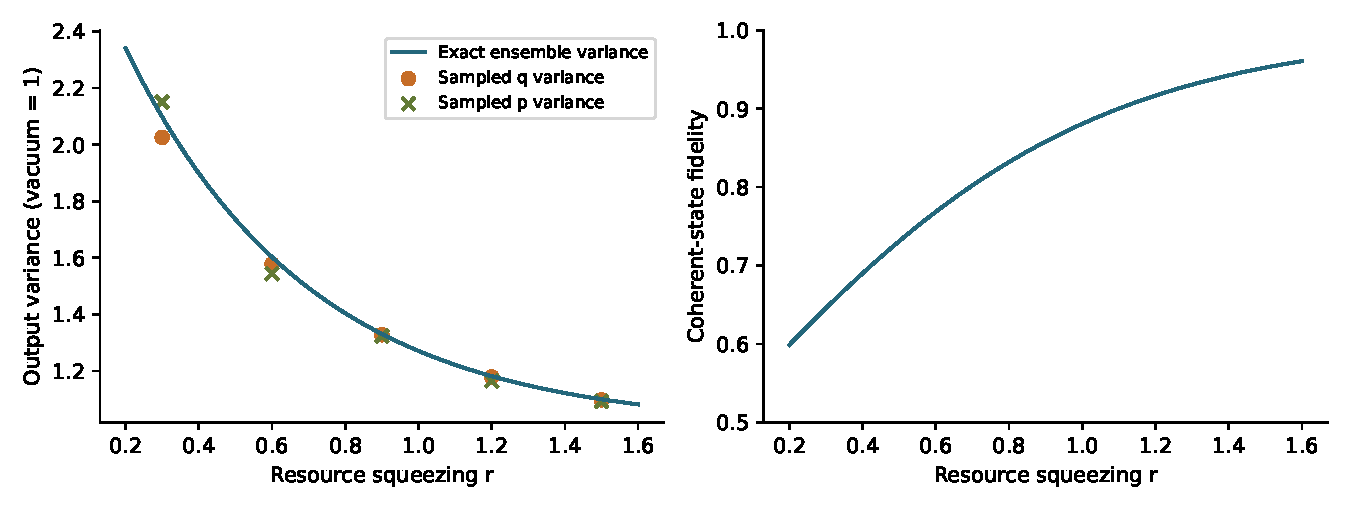
\includegraphics[width=.94\textwidth]{results/finite_squeezing.pdf}
\caption{Reproducible finite-resource identity transport. Left: the exact
unconditional output variance and two sample estimates. Right: analytic
coherent-state fidelity of the noisy identity channel. Curves are calculated
from the derived channel; markers are generated by independent trajectories.
These results are simulation data, not photonic hardware measurements.}
\label{fig:noise}
\end{figure*}

\subsection{Reproduction procedure}

The repository contains package metadata, a frozen local dependency list, CI
configuration, unit and integration tests, tutorials, example scripts, a figure
generator, source manuscript and compiled figures. The reference environment
uses Python 3.12, Piquasso 8.0.1 and GraphiX 0.4. The generated environment file
records precise NumPy, SciPy, NetworkX and plotting versions. Local CPU timings
in the CSV are provenance only; they are not cross-platform benchmarks.

\begin{lstlisting}[language=Python]
import photographiq as pg

p = pg.Circuit(1).rotate(0, 0.4).squeeze(0, 0.2)
pattern = p.compile(squeezing=1.2)
result = pg.simulate(
    pattern,
    inputs={0: pg.GaussianInput.coherent(0.3)},
    seed=42, frame=True,
)
channel = pg.gaussian_channel(pattern)
print(result.outcomes)
print(channel.matrix, channel.noise)
\end{lstlisting}

Install the development extras and run \texttt{python -m pytest}. Running
\texttt{python experiments/reproduce.py} regenerates the CSV, environment JSON,
LaTeX table and figures. The manuscript uses the official Quantum document class,
included with its original license. Running pdfLaTeX twice in the paper directory
builds the manuscript. No remote quantum service or hardware account is required.

\section{Limitations and future development}

The implementation favors explicit physics and auditability. Dense covariance
storage requires quadratic memory, and full physicality checks use dense
eigensolvers. The native adapter also copies moments between calls. Streaming
teleportation keeps the active state small, but arbitrary large graph preparation
does not yet exploit sparse covariance or specialized structure. No superiority
over optimized Piquasso execution is claimed.

The Gaussian compiler is intentionally conservative and can use many ancillas,
especially for beam splitters. Its finite-resource noise may be substantially
larger than that of specialized optical gadgets. Optimizing resource count and
noise jointly is a future task. The supplied-order CV-flow implementation does
not solve the full order-search problem. The standardizer is not a complete
CV rewrite calculus.

The stochastic execution engine converts scalar parameters to Python floats.
Symbolic construction and upstream differentiable connectors do not make it
end-to-end differentiable. Future PhotoGraphiQML work would require a dedicated
gradient-aware execution contract, estimator choices and batching support.
Gaussian fitting of adaptive mixtures must not obscure non-Gaussian ensemble
features.

Non-Gaussian resource experiments remain bounded by the explicit Fock cutoff.
Adaptive Fock homodyne, mixed-state input resources, GKP error correction,
fault-tolerant compilation and realistic temporal hardware scheduling are not
implemented. These omissions are exposed as documented capability boundaries
rather than apparently functional placeholder APIs.

\section{Conclusion}

PhotoGraphiQ provides a tested computational layer for expressing, compiling,
executing and analyzing finite-squeezing CV measurement-based computations.
Its software abstractions distinguish resource topology, measurement calculus,
classical causality and physical simulation. Independent conventions and channel
analysis make finite-resource effects visible, while raw Piquasso and structural
GraphiX tests answer different validation questions. This separation provides a
practical basis for extending Gaussian MBQC studies and carefully bounded
non-Gaussian resource experiments.

\section*{Code and data availability}
Original software is released under the MIT license at
\url{https://github.com/chinmoybiswasdeep/PhotoGraphiQ}. The local repository
contains all source and research artifacts described here; this manuscript does
not assert that the generated changes have been pushed or released remotely.
Reproduction data are in \texttt{paper/results}; research PDFs supplied for study
retain their original copyrights. The Quantum class retains its LaTeX Project
Public License. No software DOI is assigned in this draft.

\section*{Author contributions and AI-use disclosure}
The manuscript uses collective contributor metadata pending confirmation of the
actual authors and affiliations. An OpenAI Codex assistant generated the initial
software implementation, tests, documentation, calculations, figure-generation
code and manuscript text, and executed local validation. Human authors must
review the code, mathematical claims, results, references and attribution before
submission. This statement identifies the scope of AI assistance and makes no
claim about unperformed human review or experimental work.

\begin{thebibliography}{9}
\bibitem{piquasso2025}
Z. Kolarovszki, T. Rybotycki, P. Rakyta, A. Kaposi, B. Po\'or, S. J\'oczik,
D. T. R. Nagy, H. Varga, K. H. El-Safty, G. Morse, M. Oszmaniec, T. Kozsik,
and Z. Zimbor\'as,
``Piquasso: A Photonic Quantum Computer Simulation Software Platform,''
\href{https://doi.org/10.22331/q-2025-04-15-1708}{Quantum \textbf{9}, 1708 (2025)}.

\bibitem{graphix2022}
S. Sunami and M. Fukushima,
``Graphix: optimizing and simulating measurement-based quantum computation on
local-Clifford decorated graph,''
\href{https://arxiv.org/abs/2212.11975}{arXiv:2212.11975 (2022)}.

\bibitem{gu2009}
M. Gu, C. Weedbrook, N. C. Menicucci, T. C. Ralph, and P. van Loock,
``Quantum computing with continuous-variable clusters,''
\href{https://doi.org/10.1103/PhysRevA.79.062318}{Phys. Rev. A \textbf{79}, 062318 (2009)}.

\bibitem{menicucci2006}
N. C. Menicucci, P. van Loock, M. Gu, C. Weedbrook, T. C. Ralph, and M. A. Nielsen,
``Universal Quantum Computation with Continuous-Variable Cluster States,''
\href{https://doi.org/10.1103/PhysRevLett.97.110501}{Phys. Rev. Lett. \textbf{97}, 110501 (2006)}.

\bibitem{booth2023}
R. I. Booth and D. Markham,
``Flow conditions for continuous variable measurement-based quantum computing,''
\href{https://doi.org/10.22331/q-2023-10-19-1146}{Quantum \textbf{7}, 1146 (2023)}.

\bibitem{bk1998}
S. L. Braunstein and H. J. Kimble,
``Teleportation of Continuous Quantum Variables,''
\href{https://doi.org/10.1103/PhysRevLett.80.869}{Phys. Rev. Lett. \textbf{80}, 869 (1998)}.
\end{thebibliography}

\appendix
\section{Backend protocol and extension boundaries}

\texttt{BaseBackend} specifies reset, preparation, entanglement, displacement,
rotation, squeezing, beam splitting, destructive measurement and state retrieval.
Optional loss and cubic-phase operations have explicit unsupported defaults.
A backend instance passed to \texttt{simulate} is reset for each trajectory.
State interfaces use physical labels and the conventions in
Sec.~\ref{sec:conventions}, independently of native mode indices.

The Piquasso adapter constructs native Gaussian states from public moment
properties, executes native instruction programs and converts moments back.
External correlated native states can be imported with an explicit source
$\hbar$, rescaling means by $\sqrt{2/\hbar_{\mathrm{source}}}$ and native
anticommutator covariance by $1/\hbar_{\mathrm{source}}$.
This avoids treating a vacuum in one convention as a squeezed or unphysical
state in another.

Future backends must preserve destructive measurement semantics, maintain
labels after mode removal, implement deterministic seed handling, and expose
unsupported operations honestly. New covariance or Fock representations should
not leak into graph and expression modules. New optimization passes require
equivalence tests rather than assumptions based on qubit command names.

\section{Interchange, visualization and repository checks}

Pattern JSON is tagged with a schema name and version. Its decoder only constructs
an allowlist of commands, measurement descriptions, input resources and expression
nodes. Labels and tuples preserve their types. Nonfinite JSON constants and
unknown expression operations are rejected; callables are runtime-only. The
format stores computations rather than stochastic trajectories.

Resource drawings display input/output colors, labels, squeezing and edge weights.
Pattern drawings add ordered measurement annotations. Dependency drawings show
the command DAG, including quantum ordering as well as classical dependencies.
These figures are standard matplotlib artifacts suitable for export; they are
not diagrams of physical interferometer layouts.

CI configuration covers Python 3.11, 3.12 and 3.13 and includes pytest, Ruff and
wheel/source-distribution builds. Static checking uses Python 3.12 because the
installed recent NumPy type stubs use its syntax. The local run is one tested
environment, not evidence that every configured CI platform has already passed.
Source formatting, annotations, a pre-commit configuration and contribution
instructions support later extension. The supplied upstream PDFs remain study
materials, and local source checkouts are excluded from distributions.

\section{Test interpretation and numerical caution}

The raw native Gaussian sampling characterization is intentionally distinct from
a physics-correctness test. It pins an observed dependency behavior so that an
upstream change triggers review of the adapter and documentation. It should not
be read as endorsing an incorrect covariance convention. Native gate, graph and
conditional-state tests compare the properties they actually exercise.

Physicality checks use finite tolerances and cannot substitute for conditioning
analysis at extreme squeezing. The compiler checks symplectic reconstruction,
but large coefficients can still amplify finite-resource noise. CV-flow
least-squares residuals are numerical certificates for modest, well-scaled
examples; users should inspect coefficients and sensitivity for ill-conditioned
weighted graphs. A rejected order can be retried with another order, but the
software does not silently claim a global impossibility result.

Finally, normalization of a truncated Fock state preserves its use as a finite
model but does not establish convergence to an infinite-dimensional state.
Studies involving cubic phase or high squeezing should compare observables and
probabilities over increasing cutoffs and report retained norms. The Gaussian
path remains independent of this truncation and should be preferred whenever
the computation remains Gaussian.
\end{document}
